\documentclass[12pt]{article}
\usepackage{geometry}                % See geometry.pdf to learn the layout options. There are lots.
\geometry{letterpaper}                   % ... or a4paper or a5paper or ... 
%\geometry{landscape}                % Activate for for rotated page geometry
\usepackage[parfill]{parskip}    % Activate to begin paragraphs with an empty line rather than an indent
\usepackage{daves,fancyhdr,natbib,graphicx,dcolumn,amsmath,lastpage,url}
\usepackage{amsmath,amssymb,epstopdf,longtable}
\DeclareGraphicsRule{.tif}{png}{.png}{`convert #1 `dirname #1`/`basename #1 .tif`.png}
\pagestyle{fancy}
\lhead{CE 3354 -- Engineering Hydrology}
\rhead{FALL 2024}
\lfoot{ES7}
\cfoot{}
\rfoot{Page \thepage\ of \pageref{LastPage}}
\renewcommand\headrulewidth{0pt}



\begin{document}
\begin{center}
{\textbf{{ CE 3354 Engineering Hydrology} \\ {Exercise Set 7}}}
\end{center}

 \section*{\small{Exercises}}
Figure \ref{fig:RockyRun} is a Google-Earth image of some watershed.  The red boundary defines the watershed;  The distance on the image from Rain Gage R-1 to the Rocky Run Branch Gage is 1,500 feet.

\begin{figure}[h!] %  figure placement: here, top, bottom, or page
   \centering
   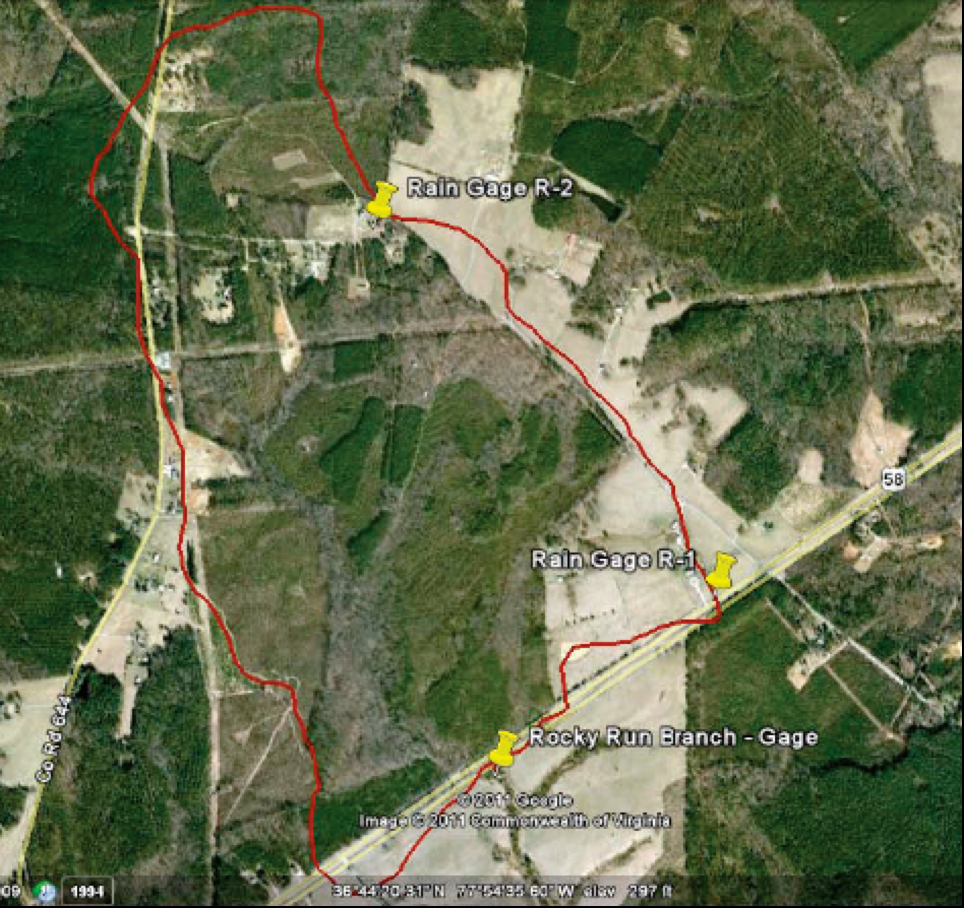
\includegraphics[width=5.0in]{RockyRun.jpg} 
   \caption{Rocky Run Branch Watershed}
   \label{fig:RockyRun}
\end{figure}

\begin{enumerate}
\item Estimate the time of concentration using the Kerby-Kirpich method assuming the slope is 0.006 along the main channel (which drains to the outlet).  The channel is clearly visible at the gage and running northward to the utility easement about 2/3 up the watershed.  Beyond the easement use your judgment as to the channel alignment. 

\textbf{Solution}

An annotated Figure \ref{fig:RockyRun} is shown below on Figure \ref{fig:RockyRunPaths}.  The blue line is main channel, it is approximately 4300 feet long using the R1 to Outlet distance as a reference distance.  The orange lines are representative overland flow paths. The flow path near R1 to outlet is at least 1500 feet (given), so will use the 1,200 foot maximum length in Kerby-Kirpich method.

\begin{figure}[h!] %  figure placement: here, top, bottom, or page
   \centering
   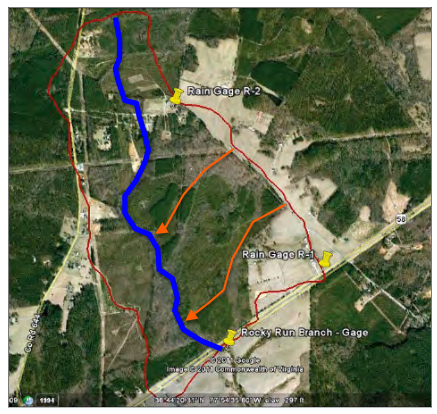
\includegraphics[width=5.0in]{RockyRunPaths.png} 
   \caption{Rocky Run Branch Watershed, Annotated with Main Channel and Overland Paths}
   \label{fig:RockyRunPaths}
\end{figure}

The overland slope would be at least equal to the channel slope (otherwise incised channel would not form) so use overland slope of 0.006. 

\begin{quote}
In hydrology, when there is evidence of an incised channel, the slopes of overland areas (overland slopes) would generally be larger than the main channel slope.

Here's why:

\begin{itemize}
\item Incised channels often indicate that the main channel has cut downward into the landscape, resulting in a deeper and flatter channel profile. The process of incision typically reduces the steepness of the main channel slope compared to surrounding areas.
\item Overland slopes are the slopes of the land surface that drain into the channel. These areas tend to be steeper because they represent the natural terrain, which hasn't undergone the same degree of erosion and flattening as the main channel.
\item Erosive processes: Overland areas experience more intense surface runoff and erosion, particularly in hilly or mountainous regions, leading to steeper slopes. In contrast, the channel, especially if incised, may have been eroded and widened over time, leading to a reduction in its gradient as it matures.
\end{itemize}
In summary, with an incised channel, the overland slopes are generally steeper than the main channel slope.
\end{quote}

Next select a retardance somewhere between Poor Grass and Pasture (N=0.3), finally apply the Kerby-Kirpich method as depicted in Figure \ref{fig:kerby}.

\begin{figure}[h!] %  figure placement: here, top, bottom, or page
   \centering
   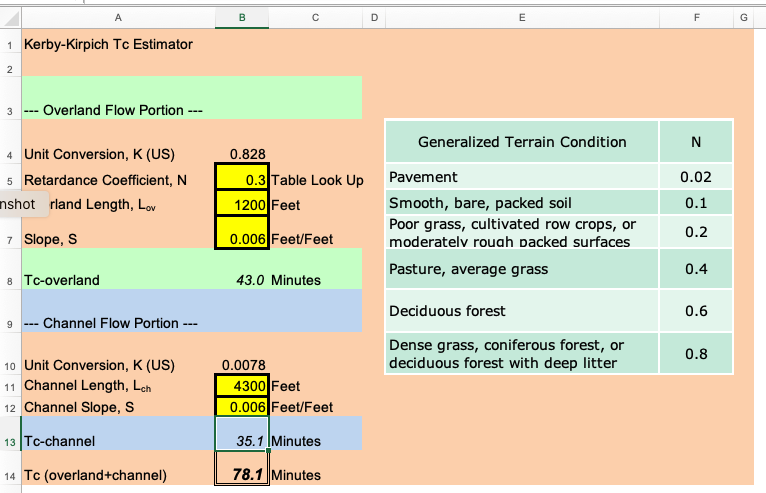
\includegraphics[width=5.0in]{Kerby.png} 
   \caption{Kerby-Kirpich Spreadsheet}
   \label{fig:kerby}
\end{figure}

The completed spreadsheet is located at \url{http://54.243.252.9/ce-3354-webroot/2-Exercises/ES-7/ES7-SourceCode/KerbyKirpich-US.xlsx}
\clearpage

\item Estimate the time of concentration using the NRCS-Upland method assuming the slope is 0.006 along the main channel (which drains to the outlet).  The channel is clearly visible at the gage and running northward to the utility easement about 2/3 up the watershed.  Beyond the easement use your judgment as to the channel alignment. 

\textbf{Solution}

An annotated Figure \ref{fig:RockyRun} is shown above on Figure \ref{fig:RockyRunPaths}.  The blue line is main channel, it is approximately 4300 feet long using the R1 to Outlet distance as a reference distance.  The orange lines are representative overland flow paths. A reasonable value is to compute two times; the main channel length and the overland flow portion.

\begin{figure}[h!] %  figure placement: here, top, bottom, or page
   \centering
   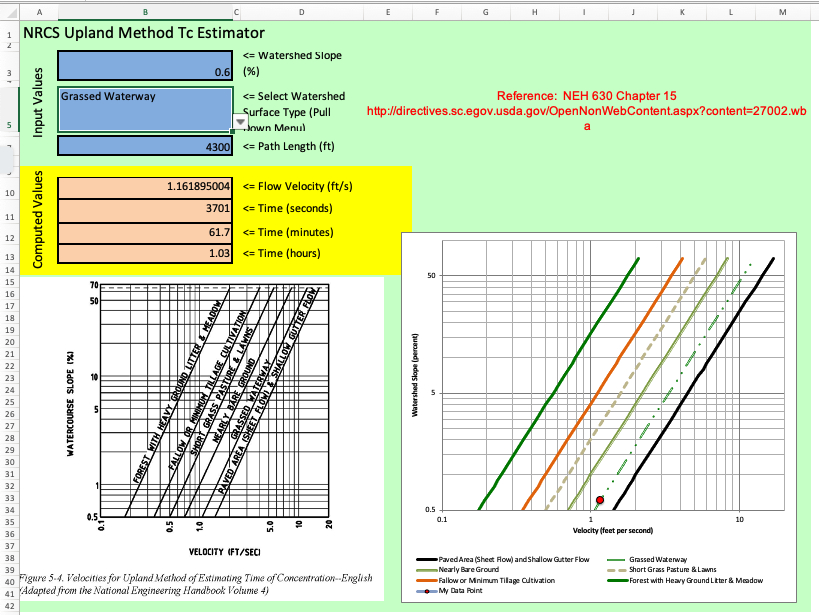
\includegraphics[width=5.0in]{NRCS-OV1.png} 
   \caption{NRCS Overland Spreadsheet}
   \label{fig:NRCS-OV1}
\end{figure}

\begin{figure}[h!] %  figure placement: here, top, bottom, or page
   \centering
   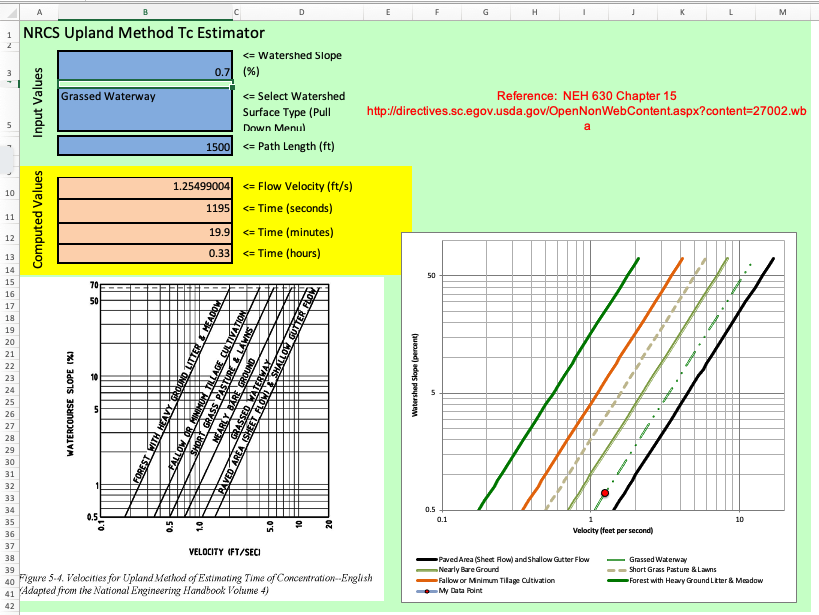
\includegraphics[width=5.0in]{NRCS-OV2.png} 
   \caption{NRCS Overland Spreadsheet}
   \label{fig:NRCS-OV2}
\end{figure}

MCL = 4300 feet; Slope =0.6\%; Time = 61.7 minutes
OVER = 1500 feet; Slope =0.7\% (an educated guess from the image); Time = 19.9 minutes

Overall time is 81.6 minutes.

\clearpage


\item Research the readings and the internet and select an additional (different) method to estimate the time of concentration -- compare the three estimates and select the estimate you would choose and explain why you would make that choice.

\begin{table}[h!]
\centering
\caption{List of Methods to Estimate $T_C$}
\begin{tabular}{p{1.5in}p{3.5in}p{1.5in}} % Column formatting, @{} suppresses leading/trailing space
~&~&~\\
Method&Best Application&Key Parameters\\
\hline
\hline
Kirpich Method&Small, steep, rural watersheds&L, S\\
TR-55 Method&Urban/rural watersheds, mixed land use&L, S, CN\\
Kinematic Wave&Overland and shallow flow&n, L, P$_2$, S\\
Bransby-Williams&Watersheds with defined channels&A, L, S\\
Kerby-Hathaway&Small, rural watersheds&L, S\\
Manning’s&Overland flow, especially in urban areas&n, L, P$_2$, S\\
Johnstone-Cross&Urban areas with shallow flow (pipes/gutters)&L, S\\
Izzard &Sheet flow over smooth/paved surfaces&L, S\\
FAA &Urban areas, especially airports&L, S, C\\
\hline
\end{tabular}
\label{tab:methods}
\end{table}

The TR-55 appears to be a good alternate method for the location, and available data. The method is summarized in Figure \ref{fig:TR55Eqn} below

\begin{figure}[h!] %  figure placement: here, top, bottom, or page
   \centering
   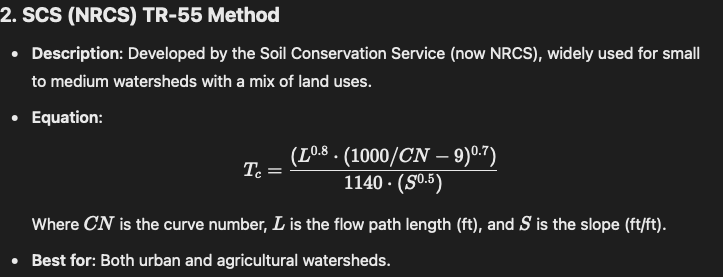
\includegraphics[width=5.0in]{TR55Eqn.png} 
   \caption{TR-55 Method}
   \label{fig:TR55Eqn}
\end{figure}

A bit subjective, but the cover suggests a HSG A or B, probably B.  The cover is pasture and woods.  Using 5800 feet as an overall path length, with a CN=50.  The time of concentration is 66 minutes.  The method is selected as pretty simple to compare to two other simple methods.

\begin{figure}[h!] %  figure placement: here, top, bottom, or page
   \centering
   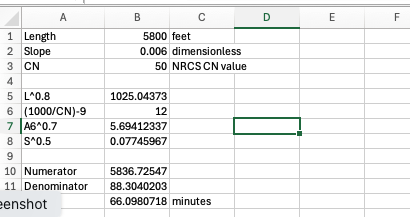
\includegraphics[width=5.0in]{Calcs.png} 
   \caption{TR-55 Calculations}
   \label{fig:Calcs}
\end{figure}

\clearpage

\item Assume the utility easment is a barrier to overland flow, and runoff can only cross at a culvert as depicted in Figure \ref{fig:RockyRunSubDivide}. The easement divides the watershed into two smaller watersheds; the upper watershed whose outlet is the culvert, and the lower watershed with same outlet as before.

\begin{figure}[h!] %  figure placement: here, top, bottom, or page
   \centering
   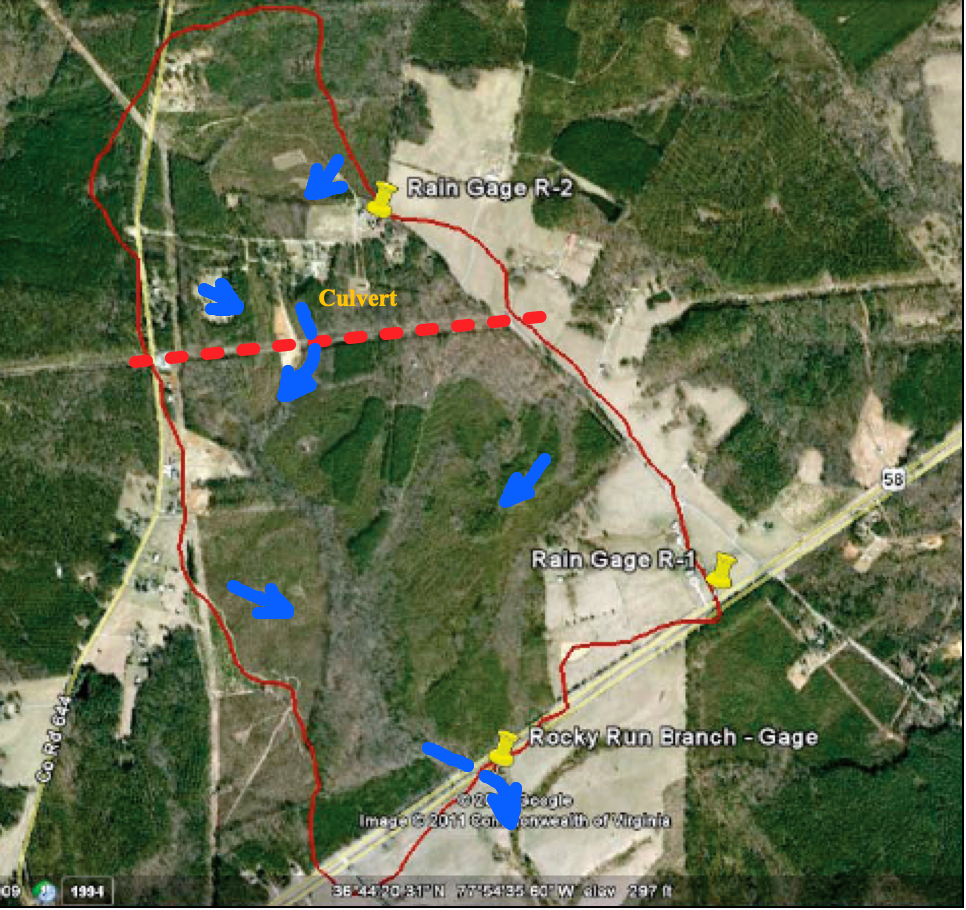
\includegraphics[width=5.0in]{RockyRunSubDivide.jpg} 
   \caption{Rocky Run Branch Watershed - Utility Easement as Barrier}
   \label{fig:RockyRunSubDivide}
\end{figure}

Estimate the time of concentration(s) using the three methods in both the upper and lower watershed.\footnote{The SCS Reservoirs in the Hardin Creek project behave similarly in that they divide the watershed into several parts which behave independently with regards to $T_C$.}

\textbf{Solution}

The main channel in the upper portion is about 1500 feet, the longest overland flow is roughly 750 feet.

The main channel in the lower portion is about 2800 feet, the longest overland flow is 1500 feet.

CN both parts is about 50 (probably bigger).  Apply the tools above to complete Table \ref{tab:TimesTable} below.

\begin{table}[h!]
\centering
\caption{List of Methods to Estimate $T_C$}
\begin{tabular}{p{2.0in}p{2.0in}p{1.0in}p{1.0in}} % Column formatting, @{} suppresses leading/trailing space
~&~&~\\
Method&Length(feet)(MC+OV)&Slope&Time(minutes)\\
\hline
\hline
Upper Basin Kerby-Kirpich&2250 &0.006&42\\
Lower Basin Kerby-Kirpich&4300 &0.006&64\\
\hline
Upper Basin Overland& 2250 &0.006&32\\
Lower Basin Overlands& 4300 &0.006&61\\
\hline
Upper Basin TR-55&2250 &0.006&29\\
Lower Basin TR-55&4300 &0.006&49\\
\hline
\end{tabular}
\label{tab:TimesTable}
\end{table}

To summarize the total $T_C$ for the two-part watershed, where all flow from upper basin passes through the culvert is 106 minutes (Kerby-Kirpich); 93 minutes (NRCS Upland); 78 minutes (TR-55).  All different, but roughly same order of magnitude.  Such variability is typical for the various methods.

%\item Estimate the watershed runoff depth using the SCS CN model for a 5-year design rainfall.  Describe how you determined the land cover conditions to select an appropriate curve number.
\end{enumerate}


%\item Blaney-Criddle San Angelo
%\item Thornwaithe San Angelo
%\item CN Concho
%\item Green-Ampt concho


\end{document}  